%%%%%%%%%%%%%%%%%%%%%%%%%%%%%%%%%%%%%%%%%%  不使用 authblk 包制作标题  %%%%%%%%%%%%%%%%%%%%%%%%%%%%%%%%%%%%%%%%%%%%%%
%-------------------------------PPT Title-------------------------------------
\title{旋转矩阵与旋-轨耦合项$\vec s\cdot\vec l$的计算}
%-----------------------------------------------------------------------------
%----------------------------Author & Date------------------------------------

%\author[\textrm{Jun\_Jiang}]{姜\;\;骏\inst{}} %[]{} (optional, use only with lots of authors)
%% - Give the names in the same order as the appear in the paper.
%% - Use the \inst{?} command only if the authors have different
%%   affiliation.
%\institute[BCC]{\inst{}%
%\institute[Gain~Strong]{\inst{}%
%\vskip -20pt 北京市计算中心}
%\vskip -20pt {\large 格致斯创~科技}}
\date[\today] % (optional, should be abbreviation of conference name)
{%	{\fontsize{6.2pt}{4.2pt}\selectfont{\textcolor{blue}{E-mail:~}\url{jiangjun@bcc.ac.cn}}}
\vskip 45 pt {\fontsize{8.2pt}{6.2pt}\selectfont{%清华大学\;\;物理系% 报告地点
	\vskip 5 pt \textrm{2023.03.24}}}
}

%% - Either use conference name or its abbreviation
%% - Not really information to the audience, more for people (including
%%   yourself) who are reading the slides onlin%%   yourself) who are reading the slides onlin%%   yourself) who are reading the slides onlineee
%%%%%%%%%%%%%%%%%%%%%%%%%%%%%%%%%%%%%%%%%%%%%%%%%%%%%%%%%%%%%%%%%%%%%%%%%%%%%%%%%%%%%%%%%%%%%%%%%%%%%%%%%%%%%%%%%%%%%

\subject{}
% This is only inserted into the PDF information catalog. Can be left
% out.
%\maketitle
\frame
{
%	\frametitle{\fontsize{9.5pt}{5.2pt}\selectfont{\textcolor{orange}{“高通量并发式材料计算算法与软件”年度检查}}}
\titlepage
}
%-----------------------------------------------------------------------------

%------------------------------------------------------------------------------列出全文 outline ---------------------------------------------------------------------------------
%\section*{}
%\frame[allowframebreaks]
%{
%  \frametitle{Outline}
%%  \frametitle{\textcolor{mycolor}{\secname}}
%  \tableofcontents%[current,currentsection,currentsubsection]
%}
%%在每个section之前列出全部Outline
%%类似的在每个subsection之前列出全部Outline是\AtBeginSubsection[]
%\AtBeginSection[]
%{
%  \frame<handout:0>%[allowframebreaks]
%  {
%    \frametitle{Outline}
%%全部Outline中,本部分加亮
%    \tableofcontents[current,currentsection]
%  }
%}

%-----------------------------------------------PPT main Body------------------------------------------------------------------------------------
\small
%\section{\rm{VASP~}软件中\rm{PAW~}计算的实现}
%\frame
%
%	\frametitle{\textrm{VASP}计算的特色}
%	相比于与普通的第一原理计算软件,\textrm{VASP}很好地平衡了计算效率和精度的问题,总的来说,\textrm{VASP}主要通过这几个特色保证了计算的高效能
%	\begin{itemize}
%	     \item 迭代与优化算法的多样性\\
%		     本质上电荷密度迭代 \textrm{\&\&} 体系总能量优化是相同的优化问题,采用了类似的算法\upcite{CMS6-15_1996,PRB54-11169_1996}:\\
%			\textcolor{blue}{\textrm{Pseudo-Newton、Conjugate-Gradient、Broyden~mix、damping-factor、RMM-DIIS}}
%	     \item 尽可能采用局域基(原子轨道基)函数:~\\
%		     \textcolor{blue}{\textrm{LREAL}}=\textcolor{red}{\textrm{.TRUE.}}\\
%			优化的投影函数也尽可能在实空间表示
%	     \item \textrm{PAW}原子数据集:\textcolor{blue}{优异的赝势}\upcite{PRB59-1758_1999}
%	\end{itemize}
%}
\section{旋转矩阵与旋-轨耦合项$\vec s\cdot\vec l$的计算}
\frame
{
	\frametitle{\textrm{Euler}角与旋转矩阵}
	从群论角度考虑,旋-轨耦合效应会引入双值群\textrm{(Double~group)}\footnote{\fontsize{5.2pt}{6.2pt}\selectfont{轨道角动量是三维空间的连续旋转本征值,可用\textrm{SO(3)}群表示;~自旋角动量则是二维复矢量的幺正群,用\textrm{SU(2)}群表示。两个群的\textrm{Lie}代数同构,但\textrm{Lie}群群元是一对二的关系。而点群都是\textrm{SO(3)}群的子群,因此不能用来描述\textrm{SU(2)}群,从而引入双值群}}

	双值群的生成元可以通过自旋轴向确定的\textrm{Euler}角确定。

	{\fontsize{6.5pt}{4.2pt}\selectfont{\textrm{WIEN2k}软件在旋-轨耦合计算时,须指定磁化轴向,由此可确定\textrm{Euler}角}}
	\begin{figure}[h!]
\centering
\vspace*{-0.21in}
\hspace*{-0.1in}
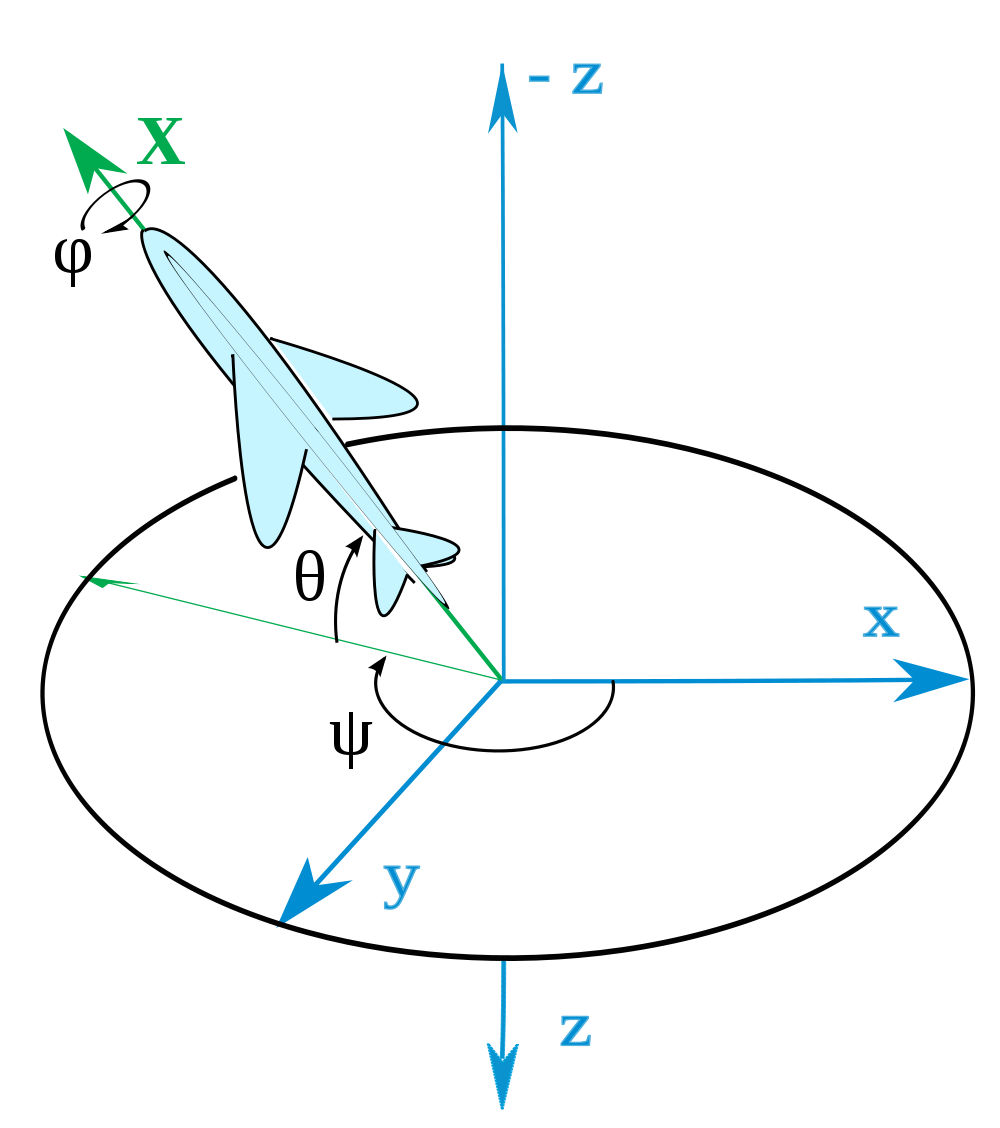
\includegraphics[height=1.7in,width=2.0in,viewport=2 5 1162 1180,clip]{Figures/euler-angles-yaw-aircraft-principal-axes-orientation-cartesian-coordinate-system.png}
\caption{\tiny \textrm{The Euler angles yaw aircraft-principal axes orientation Cartesian coordingate system.}}%(与文献\cite{EPJB33-47_2003}图1对比)
\label{Fig:Euler}
\end{figure}
}

\frame
{
	\frametitle{\textrm{Euler}角表示的旋转操作}
	{	\fontsize{6.5pt}{4.2pt}\selectfont{简要说明如下:
	旋-轨耦合引入\textrm{M\"obius}变换,用\textrm{Euler angles}表示为
	\begin{displaymath}
		\begin{aligned}
			\Pi_u(g_{\phi})=&\Pi_u\bigg[
				\begin{pmatrix}
					\cos\phi &-\sin\phi &0\\
					\sin\phi &\cos\phi &0\\
					0 &0 &1
				\end{pmatrix}
				\bigg]=&\pm
				\begin{pmatrix}
					\mathrm{e}^{\mathrm{i}\frac{\phi}{2}} &0\\
					0 &\mathrm{e}^{-\mathrm{i}\frac{\phi}{2}}
				\end{pmatrix}\\
			\Pi_u(g_{\theta})=&\Pi_u\bigg[
				\begin{pmatrix}
					1 &0 &0\\
					0 &\cos\theta &-\sin\theta\\
					0 &\sin\theta &\cos\theta
				\end{pmatrix}
				\bigg]=&\pm
				\begin{pmatrix}
					\cos\frac{\theta}{2} &\mathrm{i}\sin\frac{\theta}{2}\\
					\mathrm{i}\sin\frac{\theta}{2} &\cos\frac{\theta}{2}
				\end{pmatrix}
		\end{aligned}
	\end{displaymath}
	应用\textrm{Euler angles},可以定义旋转操作
\begin{displaymath}
		\begin{aligned}
			g(\phi,\theta,\psi)=g_{\phi}g_{\theta}g_{\psi}=
			\begin{pmatrix}
			%	\begin{aligned}
					\cos\phi &-\sin\phi &0\\
					\sin\phi &\cos\phi &0\\
					0 &0 &1
			%	\end{aligned}
			\end{pmatrix}
			\begin{pmatrix}
			%	\begin{aligned}
					1 &0 &0\\
					0 &\cos\theta &-\sin\theta\\
					0 &\sin\theta &\cos\theta
			%	\end{aligned}
			\end{pmatrix}
			\begin{pmatrix}
				\cos\psi &-\sin\psi &0\\
				\sin\psi &\cos\psi &0\\
				0 &0 &1
			\end{pmatrix}\\
			\begin{pmatrix}
				\cos\phi\cos\psi-\cos\theta\sin\phi\sin\psi &-\cos\phi\sin\psi-\cos\theta\sin\phi\cos\psi &\sin\phi\sin\theta\\
				\sin\phi\cos\psi+\cos\theta\cos\phi\sin\psi &-\sin\phi\sin\psi+\cos\theta\cos\phi\cos\psi &-\cos\phi\sin\theta\\
				\sin\psi\sin\theta &\cos\psi\sin\theta &\cos\theta
			\end{pmatrix}
		\end{aligned}
	\end{displaymath}
因此\textrm{SU(2)}群的生成元用\textrm{Euler}角表示
}}
}

\frame
{
	\frametitle{\textrm{Euler}表示的旋转操作}
	{	\fontsize{6.2pt}{4.2pt}\selectfont{
	\begin{displaymath}
		\begin{aligned}
			\Pi_u(g(\phi,\theta,\psi))=&\pm
			\begin{pmatrix}
				\mathrm{e}^{\mathrm{i}\frac{\phi}{2}} &0\\
				0 &\mathrm{e}^{-\mathrm{i}\frac{\phi}2}
			\end{pmatrix}
			\begin{pmatrix}
				\cos\frac{\theta}{2} &\mathrm{i}\sin\frac{\theta}{2}\\
				\mathrm{i}\sin\frac{\theta}{2} &\cos\frac{\theta}{2}
			\end{pmatrix}
			\begin{pmatrix}
				\mathrm{e}^{\mathrm{i}\frac{\psi}{2}} &0\\
				0 &\mathrm{e}^{-\mathrm{i}\frac{\psi}{2}}
			\end{pmatrix}\\
			=&\pm
			\begin{pmatrix}
				\cos\frac{\theta}{2}\mathrm{e}^{\mathrm{i}\frac{\phi+\psi}{2}} &\mathrm{i}\sin\frac{\theta}{2}\mathrm{e}^{\mathrm{i}\frac{\phi-\psi}{2}}\\
				\mathrm{i}\sin\frac{\theta}{2}\mathrm{e}^{-\mathrm{i}\frac{\phi-\psi}{2}} &\cos\frac{\theta}{2}\mathrm{e}^{-\mathrm{i}\frac{\phi+\psi}{2}}
			\end{pmatrix}
		\end{aligned}
	\end{displaymath}
为简化表示,习惯上将生成元记作
\begin{displaymath}
	\pm\Pi_u(g_{\alpha,\beta})=\pm
	\begin{pmatrix}
		\alpha &\beta\\
		-\overline{\beta} &\overline{\alpha}
	\end{pmatrix}
	\in\mathrm{SU(2)}
\end{displaymath}
不难看出有
\begin{displaymath}
	\begin{aligned}
		\cos\dfrac{\theta}{2}=|\alpha|,\qquad\qquad &\sin\dfrac{\theta}{2}=|\beta|, \qquad\qquad(0\leqslant\theta\leqslant\pi)\\
		\dfrac{\phi+\psi}{2}=\arg{\alpha},\qquad\qquad &\dfrac{\psi-\phi}{2}=\arg{\beta}
	\end{aligned}
\end{displaymath}
如果将$\Pi(g_{\alpha,\beta})$代入$\Pi_u(g(\phi,\theta,\psi))$则可将空间旋转操作$g(\phi,\theta,\psi)$用复数形式的$\alpha,\beta$表示为
\begin{displaymath}
	g_{\alpha,\beta}=
	\begin{pmatrix}
		\frac12\big(\alpha^2-\beta^2+\overline{\alpha^2}-\overline{\beta^2}\big) &\frac{\mathrm{i}}2\big(-\alpha^2-\beta^2+\overline{\alpha^2}+\overline{\beta^2}\big) &-\alpha\beta-\overline{\alpha}\overline{\beta}\\
		\frac{\mathrm{i}}2\big(\alpha^2-\beta^2-\overline{\alpha^2}+\overline{\beta^2}\big) &\frac12\big(\alpha^2+\beta^2+\overline{\alpha^2}+\overline{\beta^2}\big) &-\mathrm{i}\big(+\alpha\beta-\overline{\alpha}\overline{\beta}\big)\\
		\alpha\overline{\beta}+\overline{\alpha}\beta &\mathrm{i}\big(-\alpha\overline{\beta}+\overline{\alpha}\beta\big) &\alpha\overline{\alpha}-\beta\overline{\beta}
	\end{pmatrix}
\end{displaymath}
利用\textrm{Euler}角清楚地表明:~\textcolor{blue}{\textrm{SO(3)}与\textrm{SU(2)}构成满射同态群}
\begin{displaymath}
	\left\{
		\begin{aligned}
			p:~\mathrm{SU(2)}&\rightarrow \mathrm{SO(3)}\\
			\Pi_u(\pm g_{\alpha\beta})&\rightarrow g_{\alpha\beta}
		\end{aligned}
		\right.
\end{displaymath}
}}
}

\frame
{
	\frametitle{旋-轨耦合项的贡献}
	考虑旋-轨耦合后\textrm{Hamiltonian}的修正为
	\begin{displaymath}
		H_{\mathrm{SO}}=\dfrac{h}{2Mc^2}\dfrac1{r}\dfrac{\mathrm{d}V}{\mathrm{d}r}\vec{s}\cdot\vec{l}
	\end{displaymath}
%	随着磁化轴向的确定,空间\textrm{Euler}角确定,\textrm{Euler}角表示的矩阵$\Pi_u$表示局域旋转矩阵影响,具体到$\vec\sigma\cdot\vec l$项

%	对于给定的角动量$l$,
	算符$\vec{s}\cdot\vec{l}$主要作用于波函数的角度和自旋部分,即
\begin{displaymath}
	\mathrm{SO}_{m_1,m_2,\sigma_1,\sigma_2,L}=\langle\sigma_1|\langle y_{l,m_1}|\hat S\cdot\hat L|y_{l,m_2}\rangle|\sigma_2\rangle=\langle\sigma_1|\hat S|\sigma_2\rangle\langle y_{l,m_1}|\hat L|y_{l,m_2}\rangle
\end{displaymath}

因此可分别计算$\langle y_{l,m_1}|\hat l|y_{l,m_2}\rangle$和$\langle\sigma_1|\hat s|\sigma_2\rangle$:

利用升降算符与复数表示的球谐函数的关系
	{	\fontsize{8.2pt}{4.2pt}\selectfont{
\begin{displaymath}
	\begin{aligned}
		\hat{L}_-y_{l,m}=&\hbar\sqrt{l(l+1)-m(m-1)}y_{l,m-1}=&\hbar\sqrt{(l+m)(l-m+1)}y_{l,m-1}\\
		\hat{L}_+y_{l,m}=&\hbar\sqrt{l(l+1)-m(m+1)}y_{l,m+1}=&\hbar\sqrt{(l-m)(l+m+1)}y_{l,m+1}
	\end{aligned}
\end{displaymath}}}
这里$y_{l,m}$表示复数表示的球谐函数。

%电子自旋算符表示分为$|\alpha\rangle=\dfrac12\sigma$和$|\beta\rangle=-\dfrac12\sigma$%,当电子自旋与$z$方向平行时,$\mathbf{l}\cdot\mathbf{s}$将分解为
}

\frame
{
	\frametitle{旋-轨耦合项的贡献}
类似地,自旋角动量的升降算符为
\begin{displaymath}
	\begin{aligned}
		\hat S_-=&\hat S_x-\mathrm{i}\hat S_y\\
		\hat S_+=&\hat S_x+\mathrm{i}\hat S_y
	\end{aligned}
\end{displaymath}
因此直角坐标系下的自旋算符用升降算符表示为
\begin{displaymath}
	\begin{aligned}
		\hat S_x=&\dfrac12(\hat S_++\hat S_-)\\
		\hat S_y=&\dfrac1{2\mathrm{i}}(\hat S_+-\hat S_-)
	\end{aligned}
\end{displaymath}

根据上述讨论,$\vec{s}\cdot\vec{l}$可表示为:
\begin{displaymath}
%	\mathbf{l}\cdot\mathbf{s}_{\mathrm{orig}}=
	\begin{pmatrix}
		\langle\alpha|\mathrm{SO}|\alpha\rangle &\langle\alpha|\mathrm{SO}|\beta\rangle \\
		\langle\beta|\mathrm{SO}|\alpha\rangle &\langle\beta|\mathrm{SO}|\beta\rangle
	\end{pmatrix}
\end{displaymath}
这里$\mathrm{SO}$略去角动量下标,表示将$\vec s\cdot\vec l$展开后的形式
}

\frame
{
	\frametitle{旋-轨耦合项的贡献}
根据升降算符的关系,不难看出,$\vec{s}\cdot\vec{l}$的矩阵表示中
\begin{enumerate}
	\item \textcolor{blue}{电子自旋$z$方向分量,对矩阵的对角元有贡献}
	\item \textcolor{magenta}{电子自旋在$x$与$y$方向分量,将对矩阵的非对角元有贡献}
\end{enumerate}

自旋角动量是二维复矢量的幺正群,用\textrm{SU(2)}群表示,指定磁化轴向后,\textrm{SU(2)}群的生成元可由\textrm{Euler}角表示的旋转矩阵$\Pi_u$表示,
\begin{displaymath}
	\vec{s}\cdot\vec{l}= \Pi_u^{\ast}\textcolor{red}{\vec{s}\cdot\vec{l}_{\mathrm{orig}}}\Pi_u
\end{displaymath}
	{\fontsize{6.2pt}{4.2pt}\selectfont{
具体地,针对各类$l$和$s$的组合,$\vec s\cdot\vec l$矩阵的形式有(单位是$\hbar^2$)
		\begin{itemize}
			\item $\Delta m_s=0$~\&~$\Delta m =0$,矩阵对角元有贡献项,形如
	\begin{displaymath}
			\Pi_u^{\ast} 
			\begin{pmatrix}
				\dfrac{m_l}2 &0\\
				0 &\dfrac{m_l}2
			\end{pmatrix}
			\Pi_u
	\end{displaymath}
\item $|\Delta m_s|=1$~\&~$|\Delta m|=1$,矩阵非对角元有贡献项,形如
	\begin{displaymath}
		\begin{aligned}
			\Pi_u^{\ast}
			\begin{pmatrix}
			0	&\frac{\sqrt{(l+m_l)(l-m_l+1)}}2\\
			0 &0
			\end{pmatrix}
			\Pi_u\qquad\mbox{和}\qquad
			\Pi_u^{\ast} 
			\begin{pmatrix}
				0 &0\\
				\frac{\sqrt{(l-m_l)(l+m_l+1)}}2 &0
			\end{pmatrix}
			 \Pi_u
		\end{aligned}
	\end{displaymath}
		\end{itemize}
具体可根据$l,m_l,s,m_s$允许的组合依次类推
}}
}

